% ################################################################
% #                                                              #
% # Autor: Michael Epping                                        #
% # E-Mail: michael.epping@uni-muenster.de                       #
% # Version: 1.4                                                 #
% # Datum: Juni 2013                                             #
% # Info: Diese Datei sollte nicht verändert werden.             #
% #    Hier werden die Einstellungen festgelegt und              #
% #    Pakete eingebunden. Alles weitere wird über               #
% #    die Dateien verändert, die mit "0X_" beginnen.            #
% # Copyright: CC0 (macht mit diesen Dateien was ihr wollt)      #
% #    https://creativecommons.org/publicdomain/zero/1.0/deed.de #
% #                                                              #
% ################################################################

% Änderungen 1.2 -> 1.3
% * Bei der Verwendung von texlive2012 gibt es Probleme mit myalphadin.
%   Diese Vorlage für Einträge insLiteraturverzeichnis habe ich durch unsrtdin ersetzt.
% * Da ich jetzt mit TeXlipse arbeite, habe ich ein paar Anpassungen vorgenommen.
%   So ist z.B. der Name der bib-Datei fest vorgegeben, damit auch die Autovervollständigung bei BibTeX-Keys funktioniert.
% * Zusätzliche Kommentare sollten das Arbeiten mit dieser Vorlage erleichtern.
% * Die Vorlage enthält sinnvollen Text und nicht nur nutzlose Platzhalter.

% Änderungen 1.3 -> 1.4
% * Das Paket "ifthenx" gibt es unter Ubuntu 12.04 mit texlive 2009-15 nicht. Als alternative habe ich "xifthen" eingetragen.
% * Tabulatoren habe ich durch Leerzeichen ersetzt. Dadurch bleibt das Layout (Einrücken und Position Kommentare) erhalten, 
%   egal mit welchem Editor man die Dateien öffnet.
% * Ich habe einen Copyright-Vermerk hinzugefügt, nämlich dass es im Prizip keines gibt.
% * Neuer Abschnitt: latexmk
% * Neuer Abschnitt: Verbatim
% * Die Bilddatei "titelseite.jpg" wurde entfernt (wegen Copyright), da die Vorlage ab jetzt öffentlich zugänglich sein soll.
% * "README.txt" im Verzeichnis Bilder wurde erstellt.
% * Literaturangabe der Anleitung zur Optik, Wärmelehre und Atomphysik hinzugefügt. 

% ###############
% # Allgemeines #
% ###############

% Zeilen, die mit einem Prozentzeichen beginnen sind Kommentare. 
% Alle verwendeten Funktionen sind mit solchen Kommentaren versehen, so dass man den Zweck der jeweiligen Funktion nachvollziehen kann.

% ######################################
% # Konfigurieren der Dokumentenklasse #
% ######################################

\documentclass[
    a4paper,                                               % Papierformat
    oneside,                                               % Einseitig
    %twoside,                                              % Zweiseitig
    12pt,                                                  % Schriftgröße
    pagesize=auto,                                         % schreibt die Papiergröße korrekt ins Ausgabedokument
    headsepline,                                           % Linie unter der Kopfzeile
    %draft=true                                            % Markiert zu lange und zu kurze Zeilen
]{scrartcl}
% Es gibt die Dokumenttypen scrartcle, srcbook, scrreprt und scrlettr. Diese gehören zum KOME-Skript und sollten für deutsche Texte benutzt werden.
% Für englische Texte wählt man entsprechend article, book, report und letter.
% Es ist  nicht unbedingt zu empfehlen, bei einem bestehendem Dokument, die documentclass zu ändern.

% ####################
% # Pakete einbinden #
% ####################

% Pakete erweitern LaTeX um zusätzliche Funktionen. Dies ist eine Satz nützlicher Pakete.
% Weitere sollten in der Datei"`01_EigenePakete.tex"' hinzugefügt werden.
\usepackage[utf8x]{inputenc}                                                  % Legt die Zeichenkodierung fest, z.B UTF8
\usepackage[T1]{fontenc}                                                      % Verwendung der Zeichentabelle T1, für deutschsprachige Dokumente sinnvoll
\usepackage[ngerman,english]{babel}                                           % Silbentrennung nach neuer deutscher und englischer Rechtschreibung
\usepackage{amsmath}                                                          % Mathepaket
\usepackage{xifthen}                                                          % Wird benötigt um \ifthenelse zu benutzen
\usepackage[pdftex]{graphicx}                                                 % Zum flexiblen Einbinden von Grafiken, pdftex ist optional
\usepackage{units}                                                            % Ermöglicht die Nutzung von \unit[Zahl]{Einheit}
\usepackage{setspace}                                                         % Einfaches wechseln zwischen unterschiedlichen Zeilenabständen
\usepackage[pdfpagelabels]{hyperref}                                          % Verlinkt Textstellen im PDF Dokument
\usepackage[font=small,labelfont=bf,labelsep=endash,format=plain]{caption}    % Darstellung für Caption s.u.
\usepackage{subfig}                                                           % Bilder nebeneinander
\usepackage{wrapfig}                                                          % Fließtext um Figure-Umgebung
\usepackage{cite}                                                             % Zusatzfunktionen zum zitieren
\usepackage{scrpage2}                                                         % Wird für Kopf- und Fußzeile benötigt
\usepackage{array,dcolumn}                                                    % Beide Pakete werden für die Ausrichtung der Tabellenspalten benötigt

% weitere Pakete einbinden
% Die Folgenden Pakete sind schon eingebunden (siehe 00_Protokoll.tex):
% \usepackage[utf8x]{inputenc}                             % Legt die Zeichenkodierung fest, z.B UTF8
% \usepackage[T1]{fontenc}                                 % Verwendung der Zeichentabelle T1, für deutschsprachige Dokumente sinnvoll
% \usepackage[ngerman,english]{babel}                      % Silbentrennung nach neuer deutscher und englischer Rechtschreibung
% \usepackage{amsmath}                                     % Mathepaket
% \usepackage{ifthenx}                                     % Wird benötigt um \ifthenelse zu benutzen
% \usepackage[pdftex]{graphicx}                            % Zum flexiblen Einbinden von Grafiken, pdftex ist optional
% \usepackage{units}                                       % Ermöglicht die Nutzung von \unit[Zahl]{Einheit}
% \usepackage{setspace}                                    % Einfaches wechseln zwischen unterschiedlichen Zeilenabständen
% \usepackage[pdfpagelabels]{hyperref}                     % Verlinkt Textstellen im PDF Dokument
% \usepackage[font=small,labelfont=bf,labelsep=endash,format=plain]{caption}
%                                                          % Darstellung für Caption s.u.
% \usepackage{subfig}                                      % Bilder nebeneinander
% \usepackage{wrapfig}                                     % Fließtext um Figure-Umgebung
% \usepackage{cite}                                        % Zusatzfunktionen zum zitieren
% \usepackage{scrpage2}                                    % Wird für Kopf- und Fußzeile benötigt
% \usepackage{array,dcolumn}                               % Beide Pakete werden für die Ausrichtung der Tabellenspalten benötigt
\usepackage[locale = DE]{siunitx}
\usepackage[ngerman]{cleveref}
\sisetup{separate-uncertainty}

% ############################
% # Eigene Befehle einbinden #
% ############################

% Eigene Befehle eignen sich gut um Abkürzungen für lange Befehle zu erstellen. Die Syntax ist folgende:
% \newcommand{neuer Befahl}{ein langer Befehl}
% Das folgende Beispiel fügt ein Bild mit bestimmten vorgegebenen Optionen ein:
\newcommand{\cImage}[1]{
    \begin{figure}[h!]
        \centering
        \includegraphics[width=0.50\textwidth]{#1}
    \end{figure}
}
% #1 ist dabei ein Parameter, den man \cImage übergeben muss. In 10_Titelseite.tex wird dieser Befehl verwendet. Der Parameter ist dort Bilder/titelseite.jpg.
% Benötigt man keine Parameter, dann lässt man [1] weg. Werden zusätzliche Parameter benötigt, dann kann man die Zahl auf maximal 9 erhöhen.


% #########################
% # Variablen importieren #
% #########################

% Der Befehl \newcommand kann auch benutzt werden um Variablen zu definieren:

% Nummer laut Praktikumsheft:
    \newcommand{\varNum}{M1}
% Name laut Praktikumsheft:
    \newcommand{\varName}{Pendel}
% Datum der Durchführung:
    \newcommand{\varDate}{03.11.2014}
% Autoren des Protokolls:
    \newcommand{\varAutor}{Christian Mannweiler, Robin Balske}
% Nummer der eigenen Gruppe (z.B. "1mo"):
    \newcommand{\varGruppe}{Gruppe 5}
% E-Mail-Adressen der Autoren:
    \newcommand{\varEmail}{christian.mannweiler@uni-muenster.de \\ r\_bals02@wwu.de}
% E-Mail-Adresse anzeigen (true/false):
    \newcommand{\varZeigeEmail}{true}
% Literaturverzeichnis anzeigen (true/false):
    \newcommand{\varZeigeLiteraturverzeichnis}{true}
% Stil der Einträge im Literaturverzeichnis
    \newcommand{\varLiteraturLayout}{unsrtdin}

\newboolean{show}

% #########################
% # Beginn des Dokumentes #
% #########################

\begin{document}
\selectlanguage{ngerman}                                   % Schreibsprache Deutsch
\onehalfspacing                                            % 1 1/2 facher Zeilenabstand
\addtokomafont{sectioning}{\rmfamily}                      % Schriftsatz
\numberwithin{equation}{section}                           % Nummerierung der Formeln entsprechend der Section (z.B. 1.1)
\addtokomafont{caption}{\small\linespread{1}\selectfont}   % Ändert Schriftgröße und Zeilenabstand bei captions

% Römische Ziffern als Seitenzahlen für Titelseite bis einschließlich dem Inhaltsverzeichnis
\setcounter{page}{1}
\pagenumbering{roman}

% #######################################
% # Kopf- und Fußzeile konfigurieren    #
% #######################################

\ihead{\textit{\varNum\ - \varName }}                      % Innenseite der Kopfzeile
\chead{}                                                   % Mitte der Kopfzeile
\ohead{\textit{\varAutor}}                                 % Außenseite der Kopfzeile
\ifoot{}                                                   % Innnenseite der Fußzeile
\cfoot{- \textit{\pagemark} -}                             % Mitte der Fußzeile
\ofoot{}                                                   % Aussenseite der Fußzeile

% ###################################
% # Ausrichtung der Tabellenspalten #
% ###################################

\newcolumntype{,}[1]{D{,}{,}{#1}}                          % , in Tabellen untereinander stellen
\newcolumntype{p}{D{p}{\pm}{-1}}                           % +- in Tabellen untereinander stellen

% ########################
% # Titelseite einbinden #
% ########################

\begin{titlepage}
    \vspace*{4cm}
    \begin{center}
        \Huge
           \textbf{ Versuchsprotokoll {\varNum}}\\
           \varName\\
        \vspace{1cm}
        \large
        Protokoll zum Versuch Nummer {\varNum} vom \varDate \\
        \vspace{2,5cm}
        \IfFileExists{Bilder/titelseite.png}{
            \cImage{Bilder/titelseite.png}
        } % Nach \IfFileExists muss eine Leerzeile eingefügt werden

        \vspace{1,5cm}
        \varAutor \\  
        \vspace{1cm}
        \normalsize
        \textit{\varGruppe} \\
        \newboolean{showEmail}
        \setboolean{showEmail}{\varZeigeEmail}
        \ifthenelse{\boolean{showEmail}}{\textit{\varEmail}\\}{}  
    \end{center}
\end{titlepage}


% ################################
% # Inhaltsverzeichnis einbinden #
% ################################

\tableofcontents
\newpage

% Zurücksetzen der Seitenzahlen auf arabische Ziffern
\setcounter{page}{1}
\pagenumbering{arabic}

\pagestyle{scrheadings}                                    % Ab hier mit Kopf- und Fußzeile

% ###################################
% # Den Inhalt der Arbeit einbinden #
% ###################################

\section{Einleitung}

\subsection{Ziel des Versuchs}
Im Versuch M1 sollte das Verhalten verschiedener Pendel betrachtet werden.
\subsection[Physikalische Grundlagen]{Physikalische Grundlagen\footnote{Grundlagen basierend auf \cite{giancoli2010physik,tipler2008physics,anleitung-ws2014}}}

\subsubsection{Federpendel}

Am Federpendel gilt das Hooksches Gesetz $ F=-Dx $. Zusammen mit dem 2. Newton'schen Axiom ergibt sich als Bewegungsgleichung:

\begin{equation}
\label{eq1.1}
\ddot{x}+\frac{D}{m}x=0
\end{equation}

Die Lösung dieser Differentialgleichung lautet:

\begin{equation}
\label{eq1.2}
x(t)=Ae^{i\omega t}+Be^{-i\omega t}
\end{equation} 

mit $ \omega=\sqrt{\frac{D}{m}} $

\subsubsection{Fadenpendel}
 
 Beim Fadenpendel wirkt als Rückstellkraft $ F_{\varphi}=-mg\sin\varphi $
 
 Somit ist die Bewegungsgleichung mit dem zweiten Newtonschen Axiom:
 
 \begin{equation}
 \label{eq1.3}
 \ddot\varphi+\frac{g}{l} \sin\varphi =0
 \end{equation}
 Mithilfe der Kleinwinkelnäherung $\sin \varphi \approx \varphi$ vereinfacht sich diese Gleichung zu: \begin{equation}
 	 \label{eq1.3.1}
 	 \ddot\varphi+\frac{g}{l} \varphi =0
 \end{equation}
 mit der Lösung:
 
 \begin{equation}
 \label{eq1.4}
 \ddot{\varphi}(t)=Ae^{i\omega t}+Be^{-i\omega t}
 \end{equation}
 
 wobei $ \omega=\sqrt{\frac{g}{l}} $
 
 \subsubsection{gekoppelte Pendel}
 
 Bei gekoppelten Pendeln gibt es zwei Grundmoden:
 Wenn beide Pendel mit der gleichen Phase und Auslenkung schwingen gilt $ \omega_0=\omega_{gl} $.
 Wenn beide Pendel mit derselben Auslenkung und entgegengesetzter Phase schwingen gilt: $ \omega_{geg}=\sqrt{1+2D_F/D_0} $ mit $ D_0=\frac{mg}{l} $ und $D_F=D_F`\frac{l}{L}$, wobei $ D_F` $ die Federkonstante der Kopplungsfeder ist, $L$ die Gesamtlänge des Pendels und $l$ die Länge des Pendels bis zur Aufhängung der Feder.

Die Bewegungsgleichungen im Allgemeinen lauten:

\begin{align}
m\ddot x_1&=-D_0x_1-D_F(x_1-x_2)\\
m\ddot x_2&=-D_0x_2-D_F(x_1-x_2)
\end{align}

und werden durch folgende Gleichungen gelöst:

\begin{align}
x_1&=x_0\cos\left[(\frac{1}{2}\omega_{geg}-\omega_{gl} t)\right] \cdot \sin\left[ (\frac{1}{2}\omega_{geg}+\omega_{gl} t)\right] \\
x_2&=x_0sin\left[ (\frac{1}{2}\omega_{geg}-\omega_{gl} t)\right]  \cdot\sin\left[ (\frac{1}{2}\omega_{geg}+\omega_{gl} t)\right] 
\end{align}
 
Für die Periodendauer ergibt sich $ T=\frac{4\pi}{\omega_{geg}+\omega_{gl}t} $ und für die Schwebungsdauer: \\ $ T=\frac{4\pi}{\omega_{geg}-\omega_{gl}t} $

Darüber hinaus gibt es einen Kopplungsgrad, definiert durch \begin{equation}
\label{eq1.10}
k:=\frac{x_1}{x_2}
\end{equation} 

Er kann auf zwei verschiedene Arten bestimmt werden. Aus Betrachtung der Bewegungsgleichung im statischen Fall ergibt sich:

\begin{equation}
\label{eq1.11}
k=\frac{D_F}{D_0+D_F}
\end{equation}

Über die Grundfrequenzen $ \omega_{geg} $ und $ \omega_{gl} $

ergibt sich:

\begin{equation}
\label{eq1.12}
k=\frac{ \omega_{geg}^2-\omega_{gl}^2}{ \omega_{geg}^2+\omega_{gl}^2}
\end{equation}

Nach Umformung erhält man für den Quotienten aus den beiden Kreisfrequenzen:

\begin{equation}
\label{eq1.13}
\frac{\omega_{geg}}{\omega_{gl}}= \sqrt{\frac{1+k}{1-k}}
\end{equation}

und daraus für die Frequenzaufspaltung

\begin{equation}
\label{eq1.14}
\frac{\Delta\omega}{\omega_0}=\sqrt{\frac{1+k}{1-k}}-1
\end{equation}

Durch Taylorentwicklung erhalten wir als Näherung:

\begin{equation}
\label{eq1.15}
\frac{\Delta\omega}{\omega_0}=k+\frac{1}{2}k^2+\frac{1}{2}k^3
\end{equation}

%Ich würde vielleicht noch etwas zu Schwebungen schreiben, darum gings ja schließlich auch recht viel

\subsection{Stand der Literatur}

Die Normalfallbeschleunigung wurde bei  $ g_n= \SI{9,806}{m/s^2}$ festgelegt. Dieser Wert ist nicht überall gültig, da die Erde keine perfekte Kugel ist. In Anbetracht unserer Messungenauigkeiten ist er trotzdem mehr als ausreichend .
\subsection{Mess- und Auswertemethoden}
\subsubsection{Federpendel}
Die Position der Waagschale und dadurch die Auslenkung der Feder wurde durch Ablesen einer an der Wand angebrachten Skala mit 2 mm Genauigkeit durchgeführt. Die Genauigkeit aller Messungen der Auslenkung wurde mithilfe eines hinter die Waagschale gehaltenen Spiegels erhöht wodurch ein senkrechtes Ablesen gesichert wurde. Durch lang anhaltende kleine Oszillationen der Waagschale wurde die Messgenauigkeit dennoch beeinflusst, was den Fehler um schätzungsweise weitere 2 mm erhöhte. Die Massen der verwendeten Gewichte wurden von uns mit der digitalen Waage überprüft.
\subsubsection{Fadenpendel}
Der Radius der Kugel wurde über Messung des Durchmessers mit einer Schieblehre bestimmt. Die Länge der Pendelschnur wurde durch Anhalten eines Maßbandes abgelesen.
\subsubsection{gekoppeltes Pendel}
\label{messgekop zweiter änderung}
Die statische Auslenkung der beiden Pendel wurde über ein in Höhe der Pendelspitzen aufgestelltes Lineal abgelesen. Die Bestimmung der Auslenkung während der Schwingungen wurde hingegen über einen Ultraschall-Entfernungssensor vorgenommen, welcher an ein Laptop angeschlossen war. Auf diesem wurden die Messwerte in Echtzeit grafisch dargestellt. Gemessen wurde dabei der Abstand des rechten Pendels zum Entfernungssensor. Im Messprogramm war es möglich, für jede Messreihe über eine Fouriertransformation  die Frequenz der Schwingung berechnen zu lassen. Der Umgang mit dem Programm und dem Sensor gestaltete sich allerdings schwierig, da sich Einstellungen oft verstellten, das Programm abstürzte und andere unerklärliche Fehler auftraten.

\section{Versuchsdurchführung}
\subsection{Federpendel}
Bei diesem ersten Versuchsteil sollte die Federkonstante $D$ der Feder eines Federpendels auf zwei Arten bestimmt werden. Die erste Methode war die statische Bestimmung, bei welcher die Auslenkung der Feder aus der Ruhelage bei drei verschiedenen Gewichtsstücken die Grundlage der Berechnungen war. Hierzu wurde zuerst die Position der Waagschale in Ruhelage, also ohne zusätzliche Gewichtsstücke, gemessen. Danach wurden die Massestücke nacheinander auf die Waagschale gelegt und jeweils die resultierende Position erfasst. Die Differenz zur Ruheposition ergab die Auslenkung. Zuletzt wurden noch die Masse der Waagschale und der Feder bestimmt, da diese ebenfalls für die Berechnung benötigt werden.
\subsection{Fadenpendel}
Im zweiten Versuchsteil sollte die Erdbeschleunigung $g$ durch die Schwingungsdauer eines Fadenpendels bestimmt werden. Hierzu wurde das Pendel bei drei verschiedenen Längen $l$ um einen kleinen Winkel ausgelenkt und die benötigte Zeit für 50 Schwingungen gestoppt. Die Länge des Pendels wurde durch die Addition des Radius der Kugel und der Länge der Pendelschnur bestimmt.
\subsection{gekoppeltes Pendel}
Beim gekoppelten Pendel war die Aufgabe, den Kopplungsgrad $k$ und die relative Frequenzaufspaltung $\frac{\Delta \omega}{\omega_0}$ für 2 verschieden harte Federn (Kupfer und Eisen) zu bestimmen. Die Aufhängung der Feder wurde vorab auf einer Ebene ca. im zweiten Drittel der gesamten Pendellänge festgesetzt.  
\subsubsection{statische Bestimmung des Kopplungsgrades}
Die erste Art der Bestimmung von $k$ war die statische Bestimmung über die Auslenkung der Pendel. Hierzu wurde ein Pendel um $x_1=\SI{10,0+-0,2}{cm}$ von der Ruheposition ausgelenkt. Dies resultierte in folgenden Auslenkungen des gekoppelten Pendels:\\
\textbf{Kupferfeder}
$x_2=\SI{1,2+-0,4}{cm}$\\
\textbf{Eisenfeder}
$x_2=\SI{2,1+-0,4}{cm}$
\subsubsection{dynamische Bestimmung des Kopplungsgrades}
Zu Beginn der Messungen wurde sichergestellt, dass die Schwingungsdauern beider Pendel übereinstimmten. Nach einer Einführung durch den Versuchsbetreuer in den Umgang mit dem Ultraschall-Entfernungssensor wurde die Schwingungsdauer $T_0=\SI{2,48+-0,02}{s}$ eines einzelnen Pendels durch Stoppen der Dauer für 50 Schwingungen bestimmt. Dann wurde das Doppelpendel für jede Feder jeweils zu einer gleichsinnigen und gegensinnigen Schwingung angeregt. Mithilfe des Ultraschall-Entfernungssensors wurde die Schwingung aufgezeichnet. Die Periodendauer $T_{gl}$ und $T_{geg}$ konnte nun aus der vom Messprogramm berechneten Frequenz $f_{gl}$ und $f_{geg}$ berechnet werden.\footnote{Werte siehe Laborbuch} Während des Versuchs wurde von uns festgestellt, dass es schwierig war eine gleichsinnige Schwingung in Gang zu bringen, da dort Schwebungen auftraten, sodass wir mehrere Versuche benötigten um diese Schwebungen gering zu halten. Bei den gegensinnigen Schwingungen trat dieses Problem nur in einem viel geringeren Maß auf.

Als nächstes wurde das System zu Schwebungen angeregt indem ein Pendel ausgelenkt wurde, während das andere auf der Ruhelage festgehalten wurde. Wenn nun beide Pendel gleichzeitig losgelassen wurden konnten zuverlässig Schwebungen produziert werden. Bei diesem Teil des Experiments traten allerdings massive Fehler mit dem Messprogramm auf. Zusätzliche zu den in \cref{messgekop} erwähnten Problemen funktionierte die Berechnung der Frequenzen nicht mehr zuverlässig. Während bei der Eisenfeder keine Probleme auftauchten und das Programm zwei Peaks im Frequenzverlauf anzeigte welche auch mit $f_{gl}$ und $f_{geg}$ übereinstimmten, wurde uns bei der Auswertung der Kupferfeder zuerst nur ein Peak angezeigt. Auch mithilfe des Versuchsbetreuers und nach mehrmaligem erneuten Messen mit verschiedenen Abtastraten des Entfernungmessers konnte kein reproduzierbarer Frequenzverlauf erzeugt werden. Die beste Messung mit zwei Peaks (\cref %VERWEIS EINFÜGEN) 
zeigte eine ungefähre Übereinstimmung mit $f_{gl}$, der zweite Peak ist aber weit abseits des Wertes von $f_{geg}$. 

\section{Versuchsauswertung- und Ergebnisse}
\subsection{Federpendel}
Aus den gemessenen Werten und \cref{eq1.1} ergibt sich für die statische Bestimmung der Federkonstante $D=\SI{12520,5+-1954,29}{g/s^2}$

Bei der dynamischen Bestimmung der Federkonstante ergibt sich der Wert $D=\SI{12836+-17,94}{g/s^2}$
\subsection{Fadenpendel}

\subsection{gekoppeltes Pendel}
\subsubsection{statische Bestimmung des Kopplungsgrades}
\textbf{Kupferfeder}
$x_1=\SI{10,0+-0,2}{cm}$ und $x_2=\SI{1,2+-0,4}{cm}$ also ist $k=\frac{x_2}{x_1}=\SI{0,12+-0,02}{}$\\
\textbf{Eisenfeder}
$x_1=\SI{10,0+-0,2}{cm}$ und $x_2=\SI{2,1+-0,4}{cm}$ also ist $k=\frac{x_2}{x_1}=\SI{0,21+-0,02}{}$
\subsubsection{dynamische Bestimmung des Kopplungsgrades}
Aus den Periodendauern lässt sich mit \cref{eq1.12} der Kopplungsgrad bestimmen.

\textbf{Kupferfeder}\\
$T_{gl}=\SI{2,439+-0,006}{s}$ und $T_{geg}=\SI{1,960+-0,004}{s} \Rightarrow k=\SI{21,52+-0,06e-2}{}$

\textbf{Eisenfeder}\\
$T_{gl}=\SI{2,326+-0,005}{s}$ und $T_{geg}=\SI{1,695+-0,003}{s}\Rightarrow k=\SI{30,63+-0,07e-2}{}$\\
\subsubsection{Bestimmung der relativen Frequenzaufspaltung}
Die relative Frequenzaufspaltung $\frac{\Delta \omega}{\omega_0}$ ist mit $k$ aus der statischen Bestimmung und \cref{eq1.13} \\ $\frac{\Delta \omega}{\omega_0}=0,1282\pm 0,0229$ für die Kupferfeder und \\ $\frac{\Delta \omega}{\omega_0}=0,2376\pm 0,0259$ für die Eisenfeder.

Mit \cref{eq1.14} ergeben sich hingegen folgende Werte:\\
$\frac{\Delta \omega}{\omega_0}=0,1281 \pm 0,0228$ für die Kupferfeder und\\
$\frac{\Delta \omega}{\omega_0}=0,2367 \pm 0,0255 $ für die Eisenfeder.

Die benutze Näherung ist also offensichtlich sowohl beim Funktionswert als auch beim Fehlerwert bis auf die dritte Nachkommastelle genau.
\subsection{Doppelpendel}

Bei großen Winkeln verhält sich das Doppelpendel chaotisch, ohne irgendein erkennbares Muster. Bei kleineren Auslenkungen beruhigt sich dieses Verhalten und es ist eine klare Periodizität erkennbar. Dies lässt sich dadurch erklären, dass die Bewegungsgleichungen keine lineare Differentialgleichungen sind und sich das System somit auch nicht wie ein harmonischer Oszillator verhält. Bei kleinen Winkel wirkt die Kleinwinkelnäherung und die Differentialgleichungen werden linear.
\clearpage

\section{Graphische Darstellung der Ergebnisse}

Die wirklich abgelesene Frequenz in der Fouriertransformation wird durch einen Punkt angezeigt

\subsection{Kopplung durch Cu-Feder}

\begin{figure}[h!]
\centering
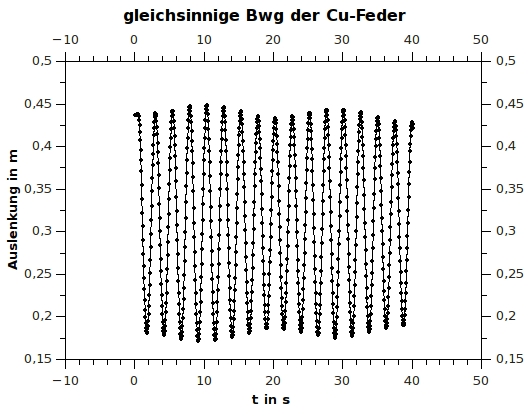
\includegraphics[width=0.6\linewidth]{../Messungen/graphen/gleich-Bwg-Cu}
\caption{Beide Pendel schwingen möglichst gleichphasig}
\label{fig:gleich-Bwg-Cu}
\end{figure}

\begin{figure}[h!]
\centering
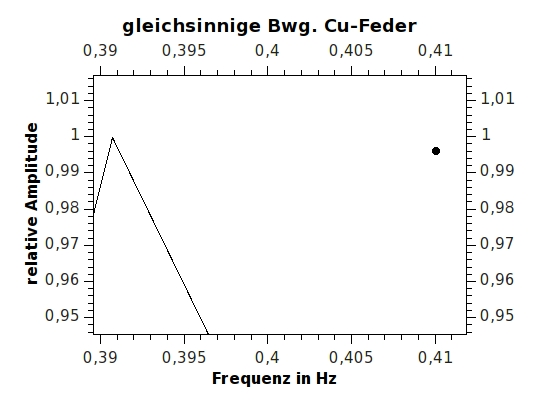
\includegraphics[width=0.55\linewidth]{../Messungen/graphen/gleich-Bwg-Cu-FFT}
\caption{Die dazugehörige Fouriertransformation}
\label{fig:gleich-Bwg-Cu-FFT}
\end{figure}

\clearpage

\begin{figure}[h!]
\centering
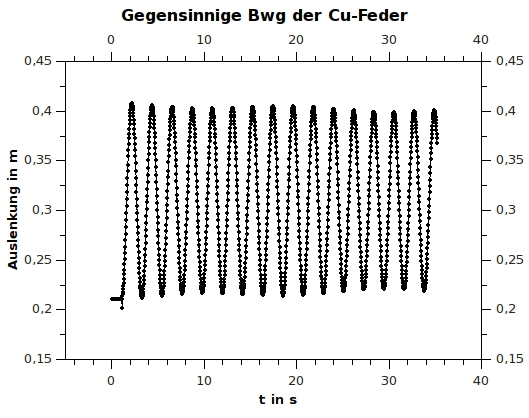
\includegraphics[width=0.55\linewidth]{../Messungen/graphen/gg-Bwg-Cu}
\caption{Beide Pendel schwingen möglichst gegenphasig}
\label{fig:gg-Bwg-Cu}
\end{figure}

\begin{figure}[h!]
\centering
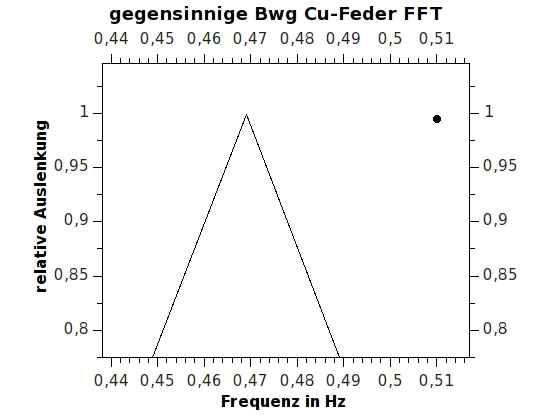
\includegraphics[width=0.7\linewidth]{../Messungen/graphen/gg-Bwg-Cu-FFT}
\caption{Die dazugehörige Fouriertransformation}
\label{fig:gg-Bwg-Cu-FFT}
\end{figure}

\clearpage
\begin{figure}[h!]
\centering
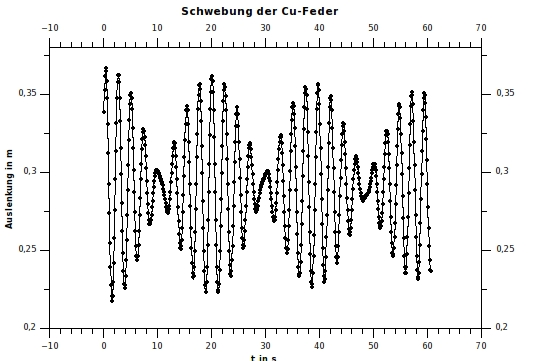
\includegraphics[width=0.7\linewidth]{../Messungen/graphen/schwebung-Bwg-Cu}
\caption{Die Pendel werden zu Schwebungen angeregt}
\label{fig:schwebung-Bwg-Cu}
\end{figure}

\begin{figure}[h!]
\centering
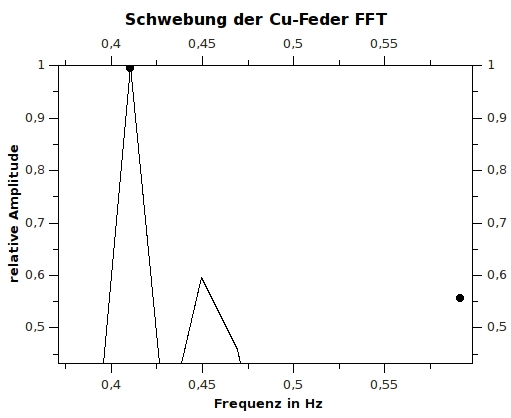
\includegraphics[width=0.7\linewidth]{../Messungen/graphen/schwebung-Bwg-Cu-FFT}
\caption{Die dazugehörige Fouriertransformation}
\label{fig:schwebung-Bwg-Cu-FFT}
\end{figure}

\clearpage

\subsection{Kopplung durch Fe-Feder}

\begin{figure}[h!]
\centering
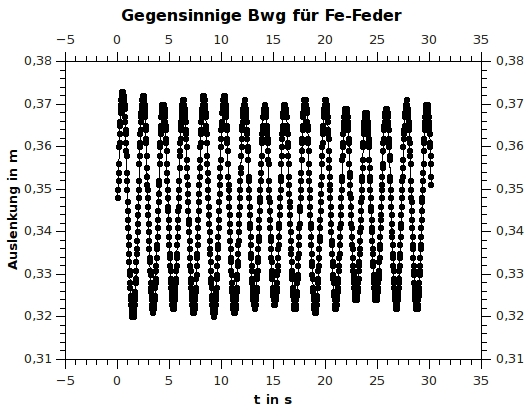
\includegraphics[width=0.65\linewidth]{../Messungen/graphen/gg-Bwg-Fe}
\caption{Die Pendel schwingen möglichst gegenphasig}
\label{fig:gg-Bwg-Fe}
\end{figure}

\begin{figure}[h!]
\centering
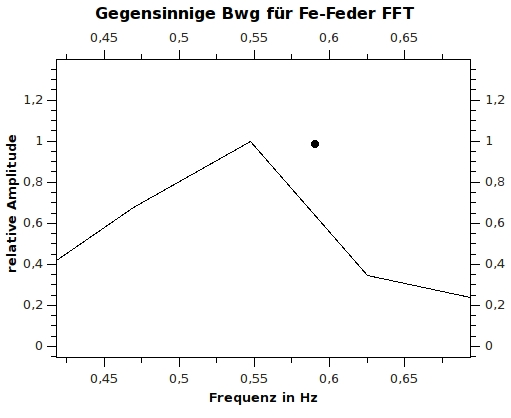
\includegraphics[width=0.7\linewidth]{../Messungen/graphen/gg-Bwg-Fe-FFT}
\caption{Die dazugehörige Fouriertransformation}
\label{fig:gg-Bwg-Fe-FFT}
\end{figure}

\clearpage

\begin{figure}[h!]
\centering
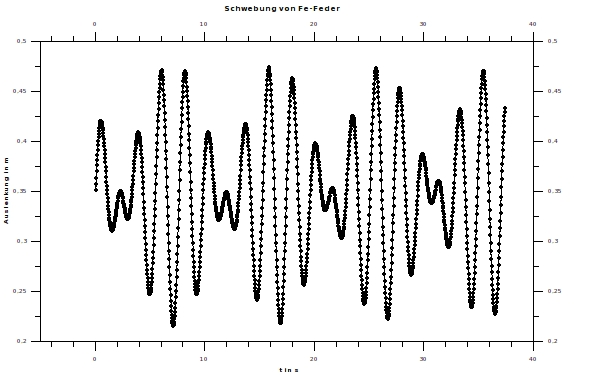
\includegraphics[width=0.7\linewidth]{../Messungen/graphen/schwebung-Fe}
\caption{Die Pendel wurden zu Schwebungen angeregt}
\label{fig:schwebung-Fe}
\end{figure}

\begin{figure}[h!]
\centering
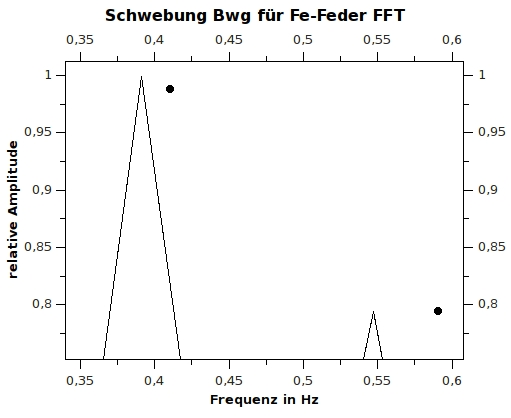
\includegraphics[width=0.7\linewidth]{../Messungen/graphen/SchwebungvonFe-FederFFT}
\caption{Die dazugehörige Fouriertransformation}
\label{fig:SchwebungvonFe-FederFFT}
\end{figure}

\clearpage

\section{Einordnung der Ergebnisse, Literaturvergleich und Diskussion}

Beim ersten Teilversuch stimmen die Ergebnisse im Fehlerbereich überein. Bei den Messungen und der Auswertung sind keine groben Fehler passiert. Man erkennt an den Fehlern, dass die statische Methode deutlich ungenauer ist als die dynamische Methode. Bei ersterem ist die statische Auslenkung aufgrund von kleinen Schwingungen nur ungenau zu bestimmen. Bei Letzterem musste nur die Periodendauer gemessen werden, was genau durchführbar ist, wenn man ie Zeit für 50 Perioden misst.

Bei der Bestimmung der Erdbeschleunigung stimmt unsere Messung mit dem Literaturwert im Fehlerbereich überein. Jedoch ist dieser Fehler mit über 10\% recht groß was auf die Vereinfachungen zurückzuführen sind. So wurde der Faden als masselos aufgefasst sowie die reale Ausdehnung der Kugel ebenso wie die Reibung vernachlässigt. Die Messung der Fadenlänge war mit dem Lineal ebenfalls ungenau.

Die Kopplungsgrade bei beiden Kopplungen stimmen nicht im Fehlerbereich überein. Die Ursache liegt in der fehlenden Kalibrierung des Ultraschallsensors sowie dem fehlerhaften Programm mit dem die Auswertung geschah. %ref müssen rein

\section{Physikalische Interpretation}

Die Messung der Erdbeschleunigung ist mit dem Fadenpendel nicht genau möglich. Es müssen zu viele Annahmen gemacht werden, als dass der reale Wert genau ermittelt werden könnte. Mit einem Federpendel (mit bekannter Federhärte) hingegen wäre die Messung viel genauer, da keine Annahmen gemacht werden müssen. Die Messfehler können durch Messung von mehreren Schwingungsperioden minimiert werden, so dass ein genauerer Wert für die Erdbeschleunigung als beim Fadenpendel bestimmt werden kann.




% ####################
% # Anhang einbinden #
% ####################

% Löscht man die Datei "`20_Anhang.tex"', dann wird kein Anhang erzeugt.
\IfFileExists{20_Anhang}{
    \newpage
    \appendix
    \section{Anhang}
\label{anhang}
\subsection{Fehlerrechnungen}
\subsubsection{Federpendel}
\textbf{statische Bestimmung der Federkonstante}:\\
$\Delta D=\sqrt{\frac{\Delta m^2 g^2}{(x_0-x)^2}+\frac{\Delta x^2 g^2 m^2}{(x_0-x)^4}}$\\
\textbf{dynamische Bestimmung der Federkonstante}:\\
$\Delta D=\sqrt{\frac{100000000 \pi ^4 \Delta m^2}{t_{50}^4}+\frac{400000000 \pi ^4 \Delta t_{50}^2 (m+36.4667)^2}{t_{50}^6}}$\\
\subsubsection{Fadenpendel}
\textbf{Länge des Fadenpendels}:\\
$\Delta l= \sqrt{\frac{\Delta l_{PS}^2}{4 \left(l_{PS}+\frac{r_K}{2}\right)}+\frac{\Delta r_K^2}{16 \left(l_{PS}+\frac{r_K}{2}\right)}}$
\subsubsection{gekoppeltes Pendel}
\textbf{statische Bestimmung des Kopplungsgrads}:\\
$\Delta k=\sqrt{(-\frac{x_2}{x_1^2}\Delta x_1)^2+(\frac{\Delta x_2}{x_1})^2}$\\
\textbf{dynamische Bestimmung des Kopplungsgrads}:\\
$\Delta k=$$\sqrt{\Delta T_{geg}^2 \left(-\frac{2 T_{geg}}{T_{geg}^2+T_{gl}^2}-\frac{2 T_{geg} \left(T_{gl}^2-T_{geg}^2\right)}{\left(T_{geg}^2+T_{gl}^2\right)^2}\right)^2+\Delta T_{gl}^2 \left(\frac{2 T_{gl}}{T_{geg}^2+T_{gl}^2}-\frac{2 T_{gl} \left(T_{gl}^2-T_{geg}^2\right)}{\left(T_{geg}^2+T_{gl}^2\right)^2}\right)^2}$\\
\textbf{relative Frequenzaufspaltung}\\

\cref{eq1.13}: $\Delta \frac{\Delta \omega}{\omega_0}=\frac{\Delta k \left(\frac{k+1}{(1-k)^2}+\frac{1}{1-k}\right)}{2 \sqrt{\frac{k+1}{1-k}}}$

\cref{eq1.14}: $\Delta \frac{\Delta \omega}{\omega_0}=\Delta k \left(\frac{3 k^2}{2}+k+1\right)$\\



} % Nach \IfFileExists muss eine Leerzeile eingefügt werden

% ###################################
% # Literaturverzeichnis mit BibTeX #
% ###################################

\setboolean{show}{\varZeigeLiteraturverzeichnis}
\ifthenelse{\boolean{show}}{
    \newpage
    \bibliography{literatur}
    \bibliographystyle{\varLiteraturLayout}
}{}

% #######################
% # Ende des Dokumentes #
% #######################

\end{document}
